\begin{figure}[t]
\centering
\begin{subfigure}{0.38\textwidth} 
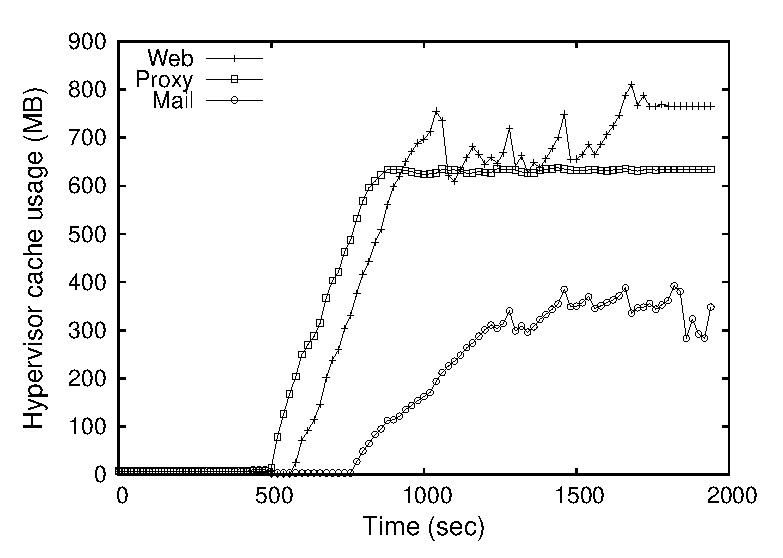
\includegraphics[width=\textwidth]{data/correctness/musage_global_new} 
 \caption{Global hypervisor cache (memory backed)}
 \label{fig:globalmem} 
\end{subfigure} 
%
\begin{subfigure}{0.38\textwidth}
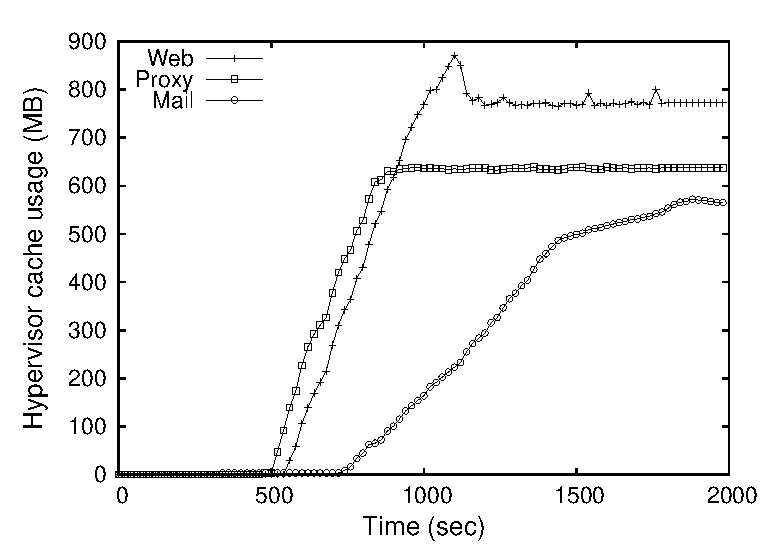
\includegraphics[width=\textwidth]{data/correctness/musage_ddecker_new} 
 \caption{\dd{} hypervisor cache (memory backed)}
 \label{fig:ddeckermem} 
\end{subfigure} 
%
\begin{subfigure}{0.38\textwidth}
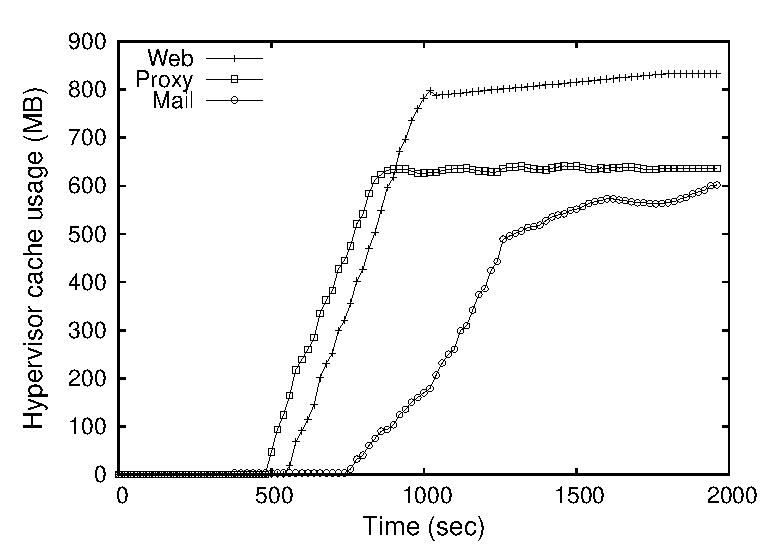
\includegraphics[width=\textwidth]{data/correctness/musage_global_ssd_new} 
 \caption{\dd{} SSD backed hypervisor cache}
 \label{fig:ddeckerssd} 
\vspace{-0.2cm}
\end{subfigure} 
%
\caption{Hypervisor cache distribution across application containers with
         different cache settings.}
\vspace{-0.25cm}
\label{fig:expt1}
\end{figure}
%{\bf Setup:} 

\section{Experimental evaluation}
\label{sec:expt}

\revised{To demonstrate the correctness of our implementation and 
showcase flexibility of \dd{} to meet memory management 
requirements of derivative clouds, we performed experiments 
using the following setup,
a 16-core blade server with 3.4 Ghz  CPUs (Intel Xeon CPU E5-2650)
and 32 GB RAM.
%
A 240GB Kingston Digital SSDNow V300 SATA 3 solid state disk, accessed
through the SATA interface.
%
As workloads, we used
the \web, \proxy, \mail{} and \video{} profiles of the 
Filebench~\cite{filebench} workload suite.}
%  
%

%\subsection{\dd{} cache size enforcement}
\subsection{Impact of caching modes}
The aim of this experiment is to establish correctness of the
two different cache store options of \dd, and to demonstrate the
benefits of partitioning the hypervisor cache.

\subsubsection{Cache size distribution}
For the experiment, a VM with 8 VCPUS and 8 GB RAM was used.
%
Four application containers (Container 1-4)  configured with 1GB RAM each,
executed the \web, \proxy, \mail, \video{} workloads.
%
All other resources (CPU and network) were allocated equally
across the application containers.  
%
Three hypervisor caching modes were compared---(i) a memory backed hypervisor cache 
with capacity 3 GB with global cache management mode, no
partitioning on a per-container basis (referred as \emph{Global}) % (\S Figure~\ref{fig:expt1}(a)), 
(ii) a 3 GB memory backed hypervisor cache with 
\dd{} cache management partitioning the cache equally among all containers
(referred as \emph{DDMem}),
%(\S Figure~\ref{fig:expt1}(b)), 
%cache management mode where every application container was assigned equal
%weightage of 25 
(iii) a 240 GB SSD backed hypervisor cache with 
\dd{} cache management partitioning the cache equally among all containers
(referred as \emph{DDSSD}).
%(\S Figure~\ref{fig:expt1}(c)). 
%cache management parwith equal weightages for each application container.
%weightage of 25 (\S Figure~\ref{fig:expt1}(c)). 
% 

\begin{figure}[t]
  \centering
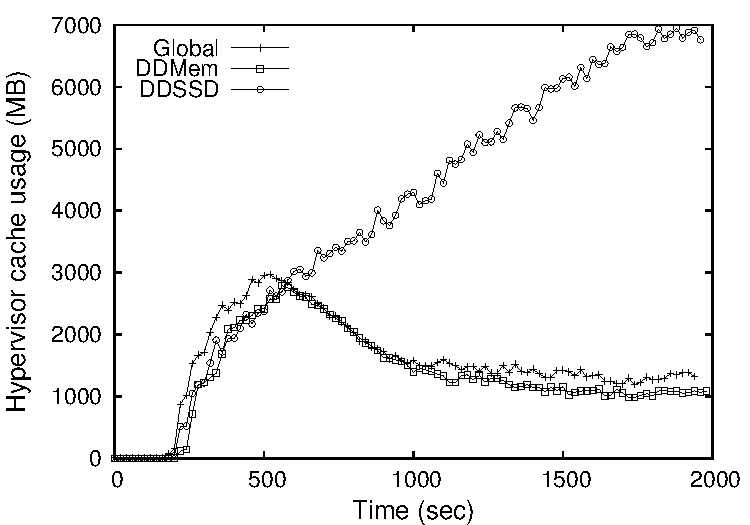
\includegraphics[width=0.38\textwidth]{data/correctness/only_video}
 \caption{\dd{} cache usage by \video-workload with different cache
          configurations.}
 \vspace{-0.5cm}
 \label{fig:video}
\end{figure} 



\begin{table*}[t]
\scriptsize
\begin{center}
\begin{tabular}{|c|c|c|c|c|c|c|c|c|c|c|c|c|}
\cline{2-13}
\multicolumn{1}{c}{} & \multicolumn{4}{|c|}{\bf Global (Memory)} & \multicolumn{4}{c|}{\bf DoubleDecker (Memory)} & \multicolumn{4} {c|}{\bf DoubleDecker (SSD)}\\
\cline{1-13}
\multicolumn{1}{|c|}{} & {\bf Throu-} & {\bf Latency} & {\bf lookup-} & {\bf \# of} & {\bf Throu-} & {\bf Latency} & {\bf lookup-}&{ \bf \# of} & {\bf Throu-} & {\bf Latency} & {\bf lookup-} & {\bf \# of}\\
%
\multicolumn{1}{|c|}{} & {\bf ghput} & {\bf (ms)} & {\bf to store} & {\bf evic-} & {\bf ghput} & {\bf (ms)} & {\bf to store}& {\bf evic-} & {\bf ghput} & {\bf (ms)} & {\bf to store} & {\bf evic-}\\
%
\multicolumn{1}{|c|}{\bf Workload} & {\bf (MB/s)} & & {\bf ratio (\%)} & {\bf -tions} & {\bf (MB/s)} & & {\bf ratio (\%)} & {\bf -tions} & {\bf (MB/s)} & & {\bf ratio (\%)} & {\bf -tions} \\
\hline
\hline
\web & 14.2 & 29.2 & 93 & 209815 & 93.7 & 3 & 99 & 0 & 5.5 & 73 & 91 & 0 \\
\hline
\proxy & 5.4 & 89.1 & 76 & 2880 & 5.6 & 85.9 & 76 & 0 & 5.2 & 91.5 & 75.9 & 0\\
\hline
Mailserver & 1.3 & 598.2 & 1 & 159793 & 1.4 & 555.7 & 32 & 0 & 2 & 386.7 & 44 & 0\\
\hline
\video & 1276 & 2.6 & 65 & 1650424 & 1188 & 2.9 & 57 & 2076672 & 481.5 & 7.8 & 67 & 0 \\
\hline
\end{tabular}
\caption{Application performance and cache behavior comparison with 
         different hypervisor caching schemes.}
\vspace{-0.7cm}
\label{table:hcache}
\end{center}
\end{table*}


Hypervisor cache distribution across the containers executing the \web, \proxy{} 
and \mail{} workloads with different caching configurations is 
shown in Figure~\ref{fig:expt1}.
%
The \video{} workload dominated the cache usage; for better presentation
cache usage of the \video{} workload with different caching modes is shown
in Figure~\ref{fig:video}.
%
As can be seen from Figure~\ref{fig:expt1} and Figure~\ref{fig:video}, 
for the first 500 seconds there is no requirement of the hypervisor cache
except for the \video{} workload. During this duration, container with
the \video{} workload occupies up to 3 GB of the cache (in all caching modes).
Beyond 500 seconds, the memory requirements of other workloads also
do not fit in the VM and the corresponding containers 
contend for the second chance cache.
Correspondingly, the \video{} workloads cache occupancy decreases from 3 GB to $\sim$ 1.4 GB.

With the global cache policy, there is no deterministic cache capacity 
for each container and all four workloads contend for the cache.
The result cache size distribution for each workload is dependent
on its access patterns and the access rate. Since \video{} workload
has the higher IO rate and quantity, it still consumes the largest
portion of the cache. The cache of the \web{} and \mail{} workloads
gets affected the most, as objects of these containers are evicted
from the cache due to pressure from the other two workloads.
In fact, the \mail{} workload gets a maximum share of less than 400 MB,
as against its fair share of 750 MB.

%With global hypervisor caching (Figure~\ref{fig:globalmem}, Figure~\ref{fig:video}), 
%\video-workload reached a cache usage peak of 
%3GB and came down to around 1.4 GB when other workloads started contending
%for the cache.
%
With \dd{} equal-weight cache partitioning (Figure~\ref{fig:ddeckermem}), 
the \video-workload was allocated ~1.2 GB when other workloads started 
using the cache up to their own entitlements. 
Since, the \proxy{} and \mail{} workloads did not consume their 
entire share of 750 MB,
the remaining capacity was shared between the \video{} and \web{} workloads.
In fact the \web{} workload does not consume more than 800 MB and hence
~1.2 GB is consumed by the \video{} workload.
%
Note that with \dd{} mode, cache usage of workloads other than \video-workload 
did not take any dips once they reached their respective peaks as opposed to
global mode.
%
This demonstrates {\em resource conservative nature} of \dd{} 
cache provisioning with {\em guaranteed isolation} according
to assigned priorities.
%
With SSD backed hypervisor caching (Figure~\ref{fig:ddeckerssd}), the cache 
size was sufficient to for all the workloads. This verified two things,
one the \dd{} could manage a SSD-based cache store correctly and
second the peak cache usage in the DDMem caching mode.
%
%So, the cache usage behavior was same with global mode and \dd{} eviction
%mode.


\subsubsection{Performance impacts with caching modes}
%Impact of cache distribution changes is shown in Table~\ref{table:hcache}.
The impact of cache distribution with different caching modes
is reported in Table~\ref{table:hcache}.
%
\web{} throughput with the DDMem caching mode (\dd{} with in-memory cache store)
was approximately {\em six times} better than the global caching mode.
%
With the \dd{}  DD-mem caching mode, \mail{} and \proxy{} workloads resulted
in marginal improvements ($\sim$5\%) and the \video-workload resulted 
in small degradation ($\sim$6\%) in application performance.
%
With the global eviction mode, evictions from workloads other than
\video{} were noticed, e.g., $\sim$200K evictions from the \web{} container. 
%
With \dd, only the \video-workload was victimized to enforce
equity at the container-level according to the equal cache distribution
configuration.

No evictions were noticed with the SSD-backed hypervisor cache % because
as the cache could host all disk cache blocks for all the
containers.
%
Because of the increased IO latency of SSD access, application
throughput for the \web{} and \video{} workloads 
was around 300\% lower compared to memory backed hypervisor cache.
%\puru{not sure how to interpret 300\% decrease.}
%\puru{to replace---decreased by 90\% and 60\% respectively.}
%
Interestingly, throughput and latency of \mail{} workload improved
by 30\% and 40\%, respectively.
%
This is due to offloading of disk operations of other workloads 
through sufficient SSD availability in the hypervisor cache.
%
These results show that even in case of sufficient hypervisor cache
availability, enforcing fairness across applications can result in
significant application benefits.
%
\revised{CPU overhead for accessing the cache in DDMem and DDSSD 
modes was comparable with the Global caching mode.
% 
In general, the overheads were equivalent to exclusive hypervisor
cache implementations in non-nested virtualized systems~\cite{kvmzcache}. 
}
\subsection{Flexible hypervisor cache management}
\label{subsec:flex}
%
\begin{table}[t]
\scriptsize
\begin{center}
\begin{tabular}{|c|c|c|c|c|}
\hline
{\bf Cache} & {\bf Webserver} & {\bf Proxycache} & {\bf Mail} & {\bf Videoserver} \\
{\bf Setting} & {\bf (C1)} & {\bf (C2)} & {\bf (C3)} & {\bf (C4)} \\
\hline 
\hline 
DDMem & Mem: 32 & Mem: 25 & Mem: 25 & Mem: 18 \\
DDMemEx & Mem: 40 & Mem: 30 & Mem: 30 & Mem: 0 \\
DDHybrid & Mem: 40 & Mem: 30 & Mem: 30 & SSD:100 \\
\hline 
\end{tabular}
\caption{\dd{} cache configuration settings.}
\vspace{-1cm}
%\puru{in previous experiment mentioned as DD-mem,etc. Fix formatting}}
\label{table:settings}
\end{center}
\end{table}
%
To analyze the effectiveness of container level priority extensions to the 
hypervisor caching, we have performed an experiment with application containers
configured with different memory limits.
%
In this experiment, the \web{} container (C1) was configured with a memory 
limit of 1.25 GB (through \cgroups) and the \video{} container (C4) was configured 
with a memory limit of 750 MB.
%
Other two containers were configured with 1 GB memory limit each.
%
The \dd{} memory cache size was limited to 2 GB.
%2 GB limit was set to the total \dd{} memory cache size,
%%which was shared by all
%the applications.
%   
In the global eviction mode (referred to as Global), only the container 
level memory limits were in action while the \dd{} hypervisor cache was 
shared globally without any container-level priority enforcement.
%
Three different cache settings (DDMem, DDMemEx and DDHybrid), shown in 
Table~\ref{table:settings}, were used to partition the \dd{} hypervisor cache
across the application containers.
%
The DDMem policy extended the \cgroup{} level memory allocation weights to the
\dd{} hypervisor cache.
%
The DDHybrid policy used the SSD store for the \video{} workload, while
containers C1-C3  shared the memory cache with weights 40, 30 and 30, respectively.
\begin{figure}[t]
  \centering
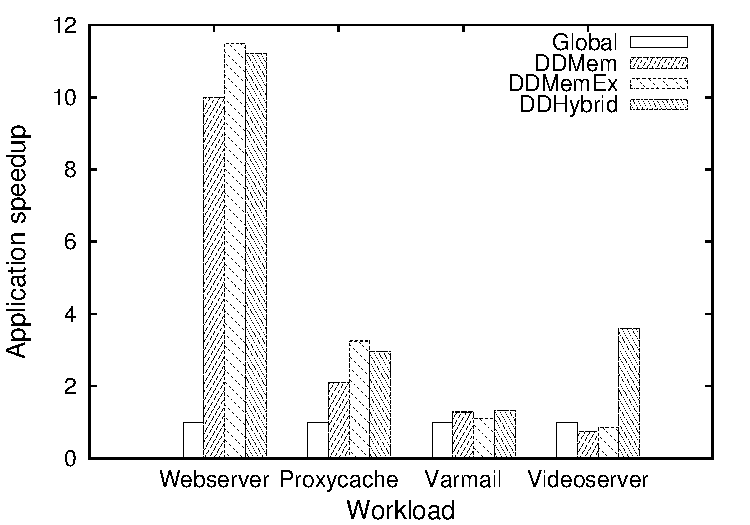
\includegraphics[width=0.43\textwidth]{data/singlevm_policy/speedup}
\vspace{-0.2cm}
 \caption{Comparison of application performance with differentiated 
          hypervisor caching policies vs. global hypervisor cache
          management.}
 \label{fig:policy_speedup}
\vspace{-0.4cm}
\end{figure} 
\begin{figure}[t]
\centering
\begin{subfigure}{0.38\textwidth} 
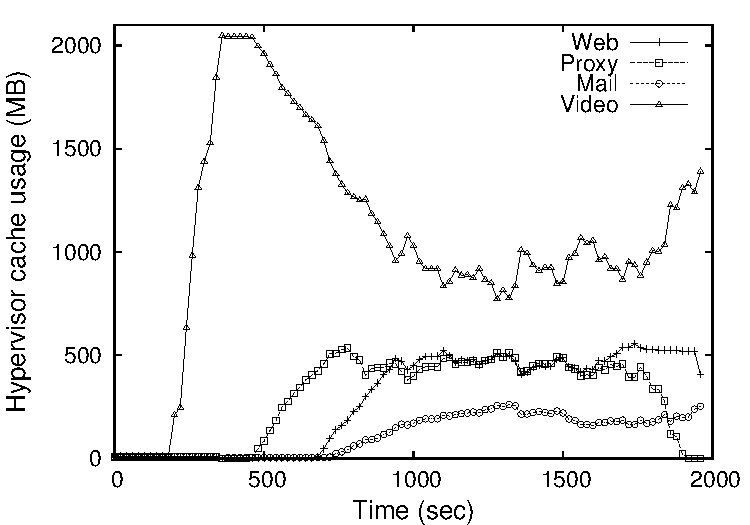
\includegraphics[width=\textwidth]{data/singlevm_policy/musage_global} 
 \caption{Global hypervisor cache}
 \label{fig:gmem1} 
\end{subfigure} 
%
\begin{subfigure}{0.38\textwidth}
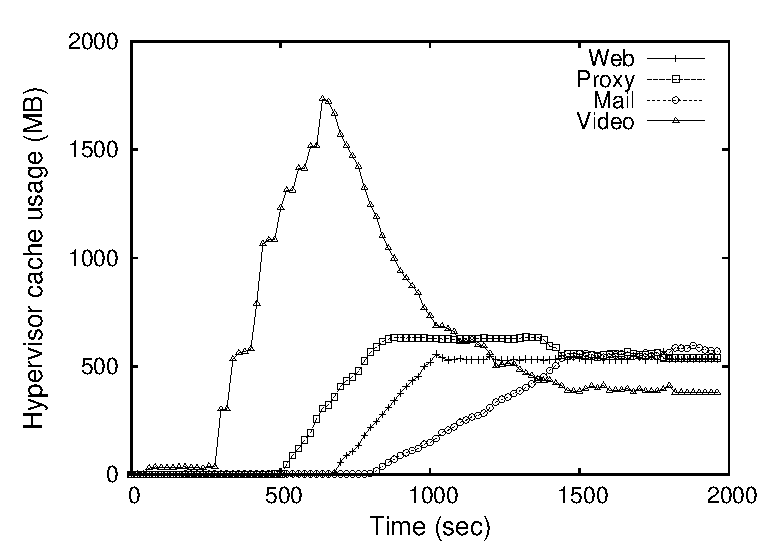
\includegraphics[width=\textwidth]{data/singlevm_policy/musage_dd_mem} 
 \caption{DDMem \dd{} policy}
 \label{fig:ddmem} 
\end{subfigure} 
%
\begin{subfigure}{0.38\textwidth}
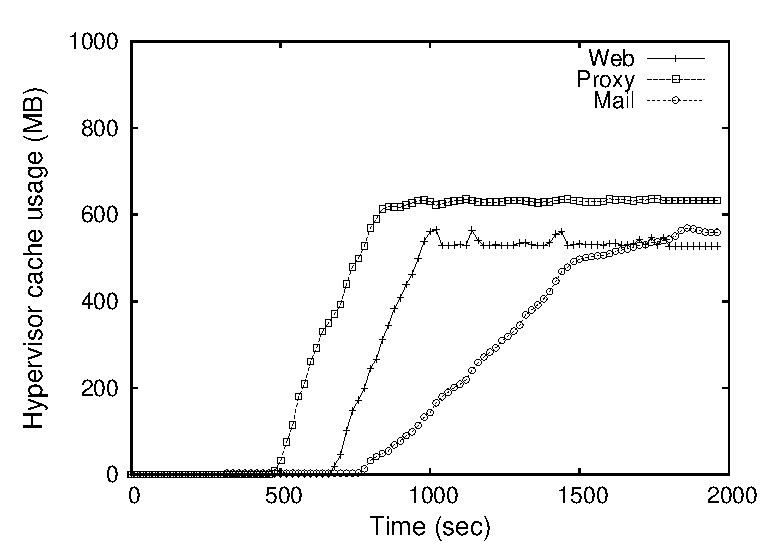
\includegraphics[width=\textwidth]{data/singlevm_policy/musage_dd_hybrid} 
 \caption{DDHybrid \dd{} policy}
 \label{fig:ddhybrid} 
\vspace{-0.2cm}
\end{subfigure} 
%
\caption{Hypervisor cache distribution across application containers with
         different cache management policies.}
\vspace{-0.7cm}
\label{fig:expt2}
\end{figure}

Application throughput improvements w.r.t the global hypervisor 
cache management mode 
and the different \dd{} caching policies is shown in Figure~\ref{fig:policy_speedup}.
%\puru{maybe unified is better than global.}
%
For the \web-workload, significant application throughput improvement
was observed---10x, 11x and 11x compared to global caching with
DDMem, DDMemEx and DDHybrid policies, respectively.
%
Around 2x, 3.2x and 3x application performance improvement resulted 
for the \proxy-workload with the three \dd{} caching modes.
%DDMem, DDMemEx and DDHybrid
%policies, respectively.
%
With the \mail{} workload, the application performance gains were marginal.
%
With the \video-workload application performance decreased with
the DDMem ($\sim$25\%) and DDMemEx ($\sim$20\%) caching modes
compared to that of the Global mode.
%
This was because the application's aggressive hypervisor cache usage 
behavior was curtailed by \dd{} policies.
%
When the \video-workload's hypervisor cache was moved to the SSD, 
3.6x improvement in application throughput was observed
compared to the global mode caching mode.

 

Hypervisor cache distribution across application containers
with the different caching modes 
as shown in Figure~\ref{fig:expt2}.
%
With the global mode, the hypervisor cache usage was dominated by the \video-workload
while other applications (C1-C3) contended for the cache
and could never reach a proportionate sharing ratio.
%
With \dd's DDMem policy, cache usage of \video-workload reduced to 
the minimum (around 400 MB), close to its fair share,
when other applications started using the cache.
%
Memory cache usage by the \web, \proxy{} and \mail{} workloads is shown in 
Figure~\ref{fig:ddhybrid} when hypervisor cache for the \video-workload 
was moved to the SSD cache (the DDHybrid mode). 
%
In this case, the 2 GB memory available for the memory backed
region of the \dd{} hypervisor cache
%configured memory backed cache of size 2GB 
was sufficient to serve all the application without resulting in 
any evictions. The three containers, each occupied about 500 MB to 600 MB
of the cache.

The main take-away from this experiment was that usage of the hypervisor cache
for different applications can be configured carefully, either to use
the memory store or the SSD store, for positive benefits for all applications.

%\puru{move figure 11 to single row.}
\subsubsection{Efficacy of cooperative memory management}
\label{subsec:coop}

%\begin{table}[t]
%\small
%\begin{center}
%\begin{tabular}{|c|c|c|c|}
%\hline
%{\bf Workload} & \bf{Technique} & {\bf Through-} & {\bf Memory} \\
% & & {\bf put (ops/sec)} & {\bf usage (GB)} \\
%\hline 
%\hline 
%{\bf MongoDB} & Morai++ & 16.9 & 0.5,1.3 \\
%%\cline{2-4}
%{\em (15 ops/sec)} & DD & 25.1 & 1,0.4 \\
%\hline
%{\bf Webserver} & Morai++ & 1289 & 2.2,0.5 \\
%%\cline{2-4}
%{\em (800 ops/sec)} & DD & 988 & 1,1.6 \\
%\hline
%{\bf Redis} & Morai++ & 13 & 1.8, 0 \\
%%\cline{2-4}
%{\em (5000 ops/sec)} & DD & 11186  & 2,0 \\
%\hline
%{\bf MySQL} & Morai++ & 48.5 & 1.6,0 \\
%%\cline{2-4}
%{\em (100 ops/sec)} & DD & 132.7 & 1.9,0 \\
%\hline 
%\end{tabular}
%\caption{\dd{} vs. centralized second chance cache management}
%\vspace{-0.5cm}
%\label{table:ddsdc}
%\end{center}
%\end{table}

\begin{table}[t]
\small
\begin{center}
\begin{tabular}{|l|c|c|c|}
\hline
{}           & {} & {} & {App. memory,}\\
{ Workload}  & { Technique} &  Throughput{} & {Hypervisor} \\
{\em (SLA)} & & { } & {cache}  \\
& & { (ops/sec)} & {(GB)}  \\
\hline 
\hline 
{\bf MongoDB} & Morai++ & 16.9 & 0.5, 1.3 \\
%\cline{2-4}
{\em (15 ops/sec)} & \dd{}& 25.1 & 1, 0.4  \\
\hline
{\bf MySQL} & Morai++ & 48.5 & 1.6, 0 \\
%\cline{2-4}
{\em (100 ops/sec)} & \dd{} & 132.7 & 1.9, 0 \\
\hline
{\bf Redis} & Morai++ & 13 & 1.8, 0 \\
%\cline{2-4}
{\em (5000 ops/sec)} & \dd{} & 11186  & 2, 0 \\
\hline
{\bf Webserver} & Morai++ & 1289 & 2.2, 0.5 \\
%\cline{2-4}
{\em (900 ops/sec)} & \dd{} & 988 & 1, 1.6  \\
\hline 
\end{tabular}
\caption{Comparison of centralized second chance cache management with \dd{}.}
\vspace{-1cm}
\label{table:ddsdc}
\end{center}
\end{table}
%To demonstrate the effectiveness of \dd{} 
%in ensuring application performance guarantees and improve overall system-wide
%performance, we performed the following experiment.
%
\dd{}, with its cooperative memory management framework, can explore 
holistic provisioning solutions that traditional centralized hypervisor
based techniques cannot.
%
To demonstrate such capabilities, we performed the following experiment.
%
A single VM hosted four application containers and executed the 
MongoDB, Redis, MySQL data stores and the Filebench Webserver workload.
The data stores acted as backends for YCSB clients.
%and
%MySQL workloads with 
The VM was provisioned with 6 GB memory and 8 CPUs (2 CPUs pinned
to each application container).
%
The hypervisor cache was provisioned to 2 GB.
%
To approximate a centralized hypervisor cache management approach 
like Morai~\cite{sdc},
we iterated over different cache partitions at the hypervisor 
cache and report
results of the best configuration (referred to as Morai++).
%
Each application had a target throughput SLA to achieve (mentioned
in the first column of Table~\ref{table:ddsdc}). The best configuration
was the one which met the individual application SLAs and yielded
the maximum aggregate throughput.
%
%we tried different cache partitioning at the hypervisor level while the VM level
%memory provisioning was left untouched.
% 

Referring to Table~\ref{table:ddsdc}, a hypervisor cache partition of 60:40 
between the MongoDB workload and the Webserver workload met their SLA requirements
and yielded the maximum aggregate throughput with Morai++.
%
Morai++ could not satisfy application performance targets of Redis and MySQL 
workloads while barely managed to meet MongoDB performance targets. 
%
In this setup, usage of the 6 GB VM memory (shared
by all containers) was 0.5 GB, 1.6 GB, 1.8 GB and 2.2 GB, for the 
MongoDB, MySQL,
Redis and Webserver workloads, respectively.
%
%The best hypervisor cache partition (referred to as Morai++)
%---adherence to minimum individual application 
%performance (Table ~\ref{table:ddsdc}, column 1) with maximum 
%global performance---is compared 
%against the best \dd{} provisioning option (referred to as DD in Table~\ref{table:ddsdc}). 
%
%when cache was partitioned in the ratio of 60:40 between MongoDB and 
%Webserver applications. 
%\puru{does not look like 60:40 in the table.}
Interestingly, with Morai++, actual hypervisor cache usage was not in the ratio of 60:40
and total average usage was below 2 GB (~1.8 GB).
%
%
%
%In all other cases of higher share allocation to MongoDB, there was no noticeable performance
%improvements for MongoDB.
%
%The average memory usage for different applications is presented in the form \textit{X,Y} in 
%Table~\ref{table:ddsdc}, where \textit{X} represents in-VM memory usage and \textit{Y} represents
%hypervisor cache usage.  
%
This was because the Webserver workload dominated the in-VM memory usage 
and did not need its maximum share of hypervisor cache leaving MongoDB-workload
to use the residual amount as per its demand (See Algorithm~\ref{algo:victim}).
%
The MongoDB workload (throttled inside the VM) could not leverage the
maximum possible hypervisor cache usage. 
%
As an additional effect, the in-VM memory usage dominance of the Webserver-workload
adversely affected other applications, notably Redis whose
working set size was ~2 GB and which did not fit in memory.
%
Note that, both Redis and MySQL applications are designed
to work only with anonymous memory and did not use the hypervisor cache
integrated with the file IO path.
%
%
%(in-VM memory) causing other
%applications to starve for memory which can not be helped by any cache partitioning scheme
%employed by Morai++.
%
With \dd{}, the VM-level manager can incorporate this information to
provision memory both from the VM and the hypervisor cache which
%
%This the main feature
the centralized hypervisor caching techniques lack. 
%
In our experiment, with \dd{}, we configured the VM memory to be allocated
as 1 GB, 2 GB, 2 GB and 1 GB, for the MongoDB, MySQL, Redis, and Webserver
workloads, respectively and discovered the best hypervisor cache
partition.
%
Based on this setup, \dd{} meets the application SLA requirements
of all the applications and the aggregate throughput achieved is higher
by a large margin.
%
This achieved primarily through improvements in the throughput achieved
by the MySQL and Redis applications.
%
Note that, both these memory-bound applications were positively 
benefited by \dd{}.
%
Also, since the working set of Redis could be accommodated in memory,
its throughput increased by a factor of 1000.


%On the other hand, 
Based on the above results, 
we demonstrate that two-level provisioning capability of \dd{} enables
holistic memory configurations which can account for application
characteristics and requirements, and yield improved application-level
and system-wide performance.
%
For workload provisioning in an adaptive manner,
\dd{} can employ well known techniques like MRC~\cite{mrc,membal},
 WSS estimation~\cite{wss,wsslow}, SHARDS~\cite{shards} etc..
%
Note that, the estimation should be done from within the VM which allows the
guest OS memory manager to provision memory resources at the two levels.
%
Centralized nesting agnostic hypervisor cache management techniques
cannot explore such provisioning configurations.
%
%space over the two levels (in-VM memory and hypervisor cache memory),
%the DD policy could meet individual application performance targets and resulted in 
%maximum system-wide benefits. 
%
\subsection{Dynamic cache management}
\begin{figure}[t]
  \centering
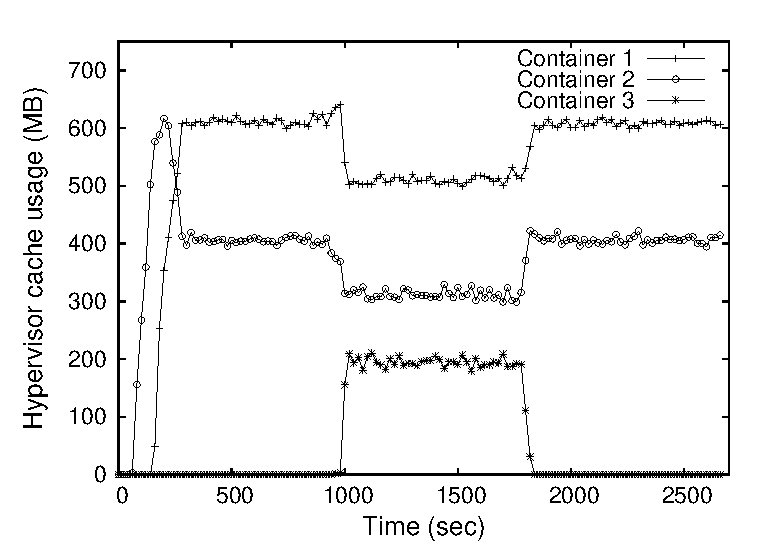
\includegraphics[width=0.38\textwidth]{data/dynamic_containers/musage}
\vspace{-0.2cm}
 \caption{Dynamic policy changes with \dd{} cache and its impact on cache 
          distribution across containers.}
\vspace{-0.55cm}
 \label{fig:dyn_distrib}
\end{figure} 
%
To demonstrate \dd's capability to apply dynamic hypervisor cache
partitioning across containers and virtual machines, we performed the
following experiments.
%
\subsubsection{Dynamic management across containers}
Initially, a single VM was configured with two application containers.
%
%
A 1 GB memory limit was configured for \dd{} memory cache while 
the SSD cache size was 240 GB.
%
Container 1 and 2 were configured with 1 GB memory each in the
virtual machine and 
executed the \web{} and \proxy{} workloads, respectively.  
%
The \dd{} cache distribution weights 
for Container 1 and 2 were set to 60 and 40, respectively.
%
After 900 seconds into the experiment, a third container (Container 3) was booted 
which executed the \video-workload.  
%
At this point, the \dd{} cache distribution weights were configured as
50, 30 and 20 for Containers 1-3, respectively.
%
After continuing with this setting for 900 seconds, the 
\video-workload (Container 3)
was configured to use the SSD store for its hypervisor cache and 
the share of Container 1 and 2 for the memory store
was reset to 60 and 40, respectively.

The \dd{} memory cache allocation across the three containers is as shown 
in Figure~\ref{fig:dyn_distrib}.
%
Initially, the cache allocation for Containers 1 and 2 were approximately 
600 MB and 400 MB,
respectively.
%
At around 1000 seconds from the start of the experiment, the \dd{} cache got 
redistributed--- $\sim$500 MB for Container 1, $\sim$300 MB  for Container 2 and
$\sim$ 200 MB for Container 3---when Container 3 started using its cache entitlement.
%
Finally, when the \dd{} cache setting for Container 3 was dynamically changed 
from memory to SSD (at around 1800 seconds), the hypervisor memory 
cache was re-distributed in the ratio of 60:40 between Container 1 and Container 2.
%
Container 3 used the SSD backed \dd{} cache for the rest of the 
experiment (not shown in Figure).
%
\dd's support for dynamic cache partitioning policies provides
flexibility in designing higher level memory management solutions. 

\subsubsection{Dynamic management across virtual machines}
\begin{figure}[t]
  \centering
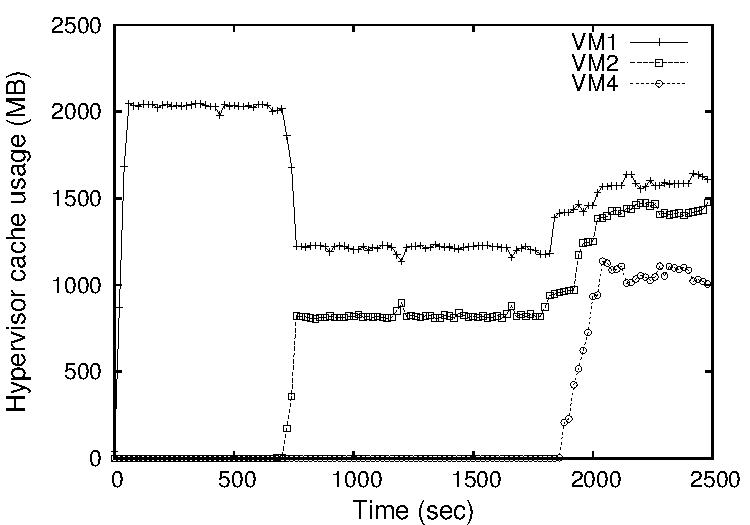
\includegraphics[width=0.38\textwidth]{data/dynamic_vms/musage}
\vspace{-0.2cm}
 \caption{Dynamic VM provisioning with policy changes triggering \dd{} cache 
          redistribution across VMs.}
\vspace{-0.25cm}
 \label{fig:vm_distrib}
\end{figure} 
In a dynamic VM provisioning setup, the number of VMs and resources
available for each change with time.
%
To demonstrate \dd's suitability in this setup, we performed the
following experiment.
%
Four VMs, each configured with 4 GB RAM were started at an
interval of 600 seconds and
each executed the \video{} workload within 
a single application container. 
%
Initially, the \dd{} memory backed cache size limit was 2 GB and VM1 
was given a weight of 100.
%
When VM2 boots up (at 600 seconds), the \dd{} cache weights 
for VM1 and VM2 were set to 60 and 40, respectively.
%
VM3 was only allowed to use the SSD cache when it started at around 1200 
seconds; VM1 and VM2 cache settings remained the same.
%
At around 1800 seconds from the start of the experiment, another
virtual machine VM4 was started.
and the \dd{} memory backed cache size was increased to 4 GB.
%
Further, the cache distribution weights for VM1, VM2 and VM4 
were configured as 40, 35 and 25, respectively.

\dd{} cache distribution across VM1, VM2 and VM4 is as shown in
Figure~\ref{fig:vm_distrib}.
%
VM1 used up the \dd{} cache entirely (2 GB) until VM2 started
using the cache (at around 650 seconds) when the cache share of
VM1 and VM2 became $\sim$1200 MB and $\sim$800 MB, respectively.
%
Instantiation of VM3 (at around 1800 seconds) did not disturb the cache
distribution between VM1 and VM2 as VM3 used the SSD cache (VM3 usage
not shown in Figure). 
%
Finally, when VM4 started and the cache capacity of \dd{} was changed 
along with cache partitioning weights, 
average cache usage of VM1, VM2 and VM4 was  
around 1600 MB, 1400 MB and 1000 MB, respectively.


With these two experiments, we demonstrated the capability of \dd{}
to dynamically manage two-levels of cache specifications in a
dynamic manner. Policy decision at the hypervisor which effect
VM-level cache partitioning and decisions that effect the
per-container partition sizes for each VM can be handled by \dd{}
in a dynamic manner. This feature is a key enabler to develop
adaptive memory and cache management policies depending
on application behavior, workloads and execution entity priorities.
%
\revised{
\subsection{Dynamic policy considerations}
%
In a dynamic scenario, mapping high level policy objectives into DoubleDecker's
weight based memory/SSD provisioning is non-trivial.
%
From the VM-level resource manager perspective, \dd{} can provide 
information regarding the available cache size and cache utility aspects
of existing application containers (GET\_STATS operation, see \S\ref{sec:impl}).
%
Any change in caching resource at the hypervisor (because of
new VMs provisioned or released), or change in application container profile in
the VM, or application SLA requirement
should trigger a readjustment of \dd{} cache usage weights.
%
%
%\deba{should we add control theoritic work like centaur and tws here?}
%Existing techniques like MRC~\cite{mrc,membal,tws}, WSS estimation~\cite{wss, shards, centaur} etc. 
%to model the relationship between memory allocation and application performance 
%can be incorporated in our system.
Existing techniques based on working set size estimation~\cite{wss, shards, tws} 
and miss-ratio-curves ~\cite{mrc,membal,centaur} which model the relationship between
memory allocation and application performance can be incorporated in our system.
%
Further, given the VM-level policy controller's access to information 
regarding resource availability and application performance, {\em both in-VM and
at the hypervisor}, new holistic policy directions can be explored.
%
We envision immediate future work of \dd{} to design such
holistic policies and
address requirements of dynamic setups at scale.
%We understand the need for realistic setups (workloads, scale etc.) to evaluate
%such dynamic policies and leave this as part of our future work. 
}
%
